\documentclass[12pt]{article}

\usepackage{natbib,amsfonts,graphics,amsmath}
\usepackage{graphicx}

\include{newcommands}

\begin{document}

\title{Derivation of the nondimensional lee wave equations and perturbation expansions}

\author{Oliver Fringer and Eric Mayer}

\maketitle

\section{Dimensional analysis}

The form drag $F$ (per unit width) due to a hill of height $h_0$ in an infinitely 
deep fluid is characterized by the dimensional quantities
$U$, $k$, $N$, and $h_0$.  Choosing $U$ and $N$ to nondimensionalize $k$ and $h_0$, the governing
nondimensional parameters are $J = N h_0/U$ and $\epsilon = k U/N$.  Since the units of the form drag
are length$^3$~time$^{-2}$, then a scale for $F$ in terms of $U$ and $N$ is $\rho_0 U^3 N^{-1}$. Therefore,
the form drag must satisfy
\[
\frac{F}{\rho_0 U^3 N^{-1}} = f(J, \epsilon)\,.
\]

\section{Nondimensional equations} \label{eq:equations}

Let $\ub_{\mbox{total}} = U {\bf e}_x + \ub$, $\rho_{\mbox{total}} = \rhobar(z) + \rho$, and
$p_{\mbox{total}} = \rho_0 \overline{p}(z) + \rho_0 p$ (the total notation is
to avoid carrying around the prime, but in a paper you should carry around the prime).
The steady momentum and density transport equations are given by
\begin{eqnarray}
U \D{u}{x} + \ub\cdot\nabla u &=& -\D{p}{x}\,,\\
U \D{w}{x} + \ub\cdot\nabla w &=& -\D{p}{z} - \frac{\rho}{\rho_0} g\,,\\
U \D{\rho}{x} + \ub\cdot\nabla\rho &=& \frac{\rho_0 N^2}{g} w\,,
\end{eqnarray}
where $N^2 = -g/\rho_0 \partial\rhobar/\partial z$, subject to continuity $\nabla\cdot\ub=0$ and
the kinematic bottom boundary condition
\[
U\D{h}{x} + u \D{h}{x} = w\,.
\]  
Nondimensionalize with
\begin{eqnarray*}
u &=& u_0 u^*\,,\\
w &=& w_0 w^*\,,\\
\rho &=& R \rho^*\,,\\
p &=& P p^*\,,\\
x &=& k^{-1} x^*\,,\\
z &=& \delta z^*\,.
\end{eqnarray*}
Nondimensionalizing the kinematic bottom boundary condition gives
(after ignoring the $*$)
\[
k U h_0 \D{h}{x} + k u_0 h_0 \D{h}{x} = w_0 w\,.
\]
If we require a balance between the linear terms, this implies $w_0 = k h_0 U$, so that
\[
\D{h}{x} + F \D{h}{x} = w\,,
\]
where $F = u_0/U$ is a Froude number. Now, the vertical scale of the flow as given by $\delta$ is not the
same as the hill height $h_0$, since $\delta$ must be finite as $h_0\to 0$ (the linear limit). The 
vertical scale is thus dictated by continuity, which requires
\[
k u_0 \D{u}{x} + \frac{w_0}{\delta} \D{w}{z} = 0\,,
\]
or, since this implies $k u_0 = w_0/\delta$, then we must have $\delta = w_0/(k u_0) = k h_0 U/(k u_0) = F^{-1} h_0$.
Nondimensionalizing the $u$-momentum equation,
\begin{eqnarray}
k u_0 U \D{u}{x} + k u_0^2\ub\cdot\nabla u  &=& -k P \D{p}{x}\,.
\end{eqnarray}
Since we require a leading-order balance between the pressure gradient and the linear momentum advection term,
we must have $P = u_0 U$, which gives
\begin{eqnarray}
\D{u}{x} + F \ub\cdot\nabla u &=& -\D{p}{x}\,.
\end{eqnarray}
The nondimensional density transport equation is given by
\[
k U R \D{\rho}{x} + k u_0 R \ub\cdot\nabla\rho = \frac{k \rho_0 h_0 N^2 U}{g} w\,.
\]
If we require a balance between the linear advection terms, then the scale for the density
perturbation is 
\[
R = \frac{\rho_0 N^2 h_0}{g}\,,
\]
so that the nondimensional density equation is
\[
\D{\rho}{x} + F \ub\cdot\nabla\rho = w\,.
\]
Nondimensionalizing the vertical momentum equation, we have
\[
k^2 h_0 U^2 \D{w}{x} + k^2 h_0 u_0^2\ub\cdot\nabla w = -\frac{P}{\delta}\D{p}{z} - \frac{g R}{\rho_0} \rho\,.
\]
If we require a vertical hydrostatic balance to leading order, then we must have 
\[
\frac{P}{\delta} = \frac{g R}{\rho_0} 
  = N^2 h_0\,,
\]
and
\[
P = \delta N^2h_0
= \frac{N^2h_0^2}{F}
= \frac{N^2h_0^2U}{u_0}.
\]
%\[
%P = \frac{g R \delta}{\rho_0} 
%  = \frac{g}{\rho_0} \frac{\rho_0 N^2 h_0}{g} \frac{h_0}{F}
%  = \frac{g}{\rho_0} \frac{\rho_0 N^2 h_0}{g} \frac{U}{N}
%  = U N h_0\,.
%\]
which gives
\[
\epsilon^2 \left(\D{w}{x} + F\ub\cdot\nabla w\right) = -\D{p}{z} - \rho\,,
\]
where 
\[
\epsilon = \frac{k U}{N}
\]
is the nonhydrostatic parameter. Now, returning to the pressure, since from the vertical momentum equation we
require $P = N^2h_0^2U u_0^{-1}$ and from the horizontal momentum equation we require $P = u_0 U$, then equating the
two implies that $u_0 = N h_0$ and the Froude number is given by
\[
F = \frac{u_0}{U} = \frac{N h_0}{U} = J\,,
\]
where
\[
J = \frac{N h_0}{U}\,.
\]
Therefore, in terms of $J$, the governing nondimensional equations are given by
\begin{eqnarray*}
\D{u}{x} + J\ub\cdot\nabla u &=& -\D{p}{x}\,,\\
\epsilon^2 \left(\D{w}{x} + J\ub\cdot\nabla w\right) &=& -\D{p}{z} - \rho\,,\\
\D{\rho}{x} + J \ub\cdot\nabla\rho &=& w\,,
\end{eqnarray*}
subject to $\nabla\cdot\ub=0$ and the kinematic bottom boundary condition
\[
\left(1 + J \right)\D{h}{x} = w\,.
\]
These nondimensional equations are consistent with the original nondimensionalization which implied
that the problem is uniquely characterized by $\epsilon$ and $J$.
The relevant scales (nondimensionalized by $N$ and $U$) are given by
\begin{eqnarray*}
\frac{u_0}{U} &=& J\,,\\
\frac{w_0}{U} &=& \epsilon J\,,\\
\frac{gR}{\rho_0 U N} &=& J\,,\\
\frac{P}{U^2} &=& J\,,\\
\frac{\delta N}{U} &=& 1\,.
\end{eqnarray*}

Contrary to what is stated in the literature, we can show that it is
in fact appropriate to refer to $J$ as an internal Froude number. If we define
$Fr_\delta = u_0/\sqrt{g' \delta}$, where $g'\delta =g (R/\rho_0) \delta = J U^2$, this gives
$Fr_{\delta} = J^{1/2}$. Therefore, $J^{1/2}$ can be thought of as 
the ratio of the inertial to gravitational forces arising from the perturbed
flow above the hill. Although we would expect a larger $N$ to block the flow and
reduce the magnitude of the perturbation above the hill, the scaling shows that
$u_0 = J U$, implying that the perturbation velocity above the sill increases in step with
increasing $J$. However, the gravitational force resulting from the perturbation is
given by $\sqrt{g'\delta} = J^{1/2} U$, which grows more slowly than $u_0$ with
increasing $J$.

This identification of J as the internal froude number squared appears to have gone without notice in the 65 years of studying Long's model. However, an inquiry into the upper limit of this relationship recently emerged from consideration of blocked flow past a half cylinder (Winters and Armi, 2012). In the blocked regime, that is, for flow in which $J>1$, the lowest fluid elements upstream of the obstacle lack sufficient kinetic energy to overtop the obstacle, and thus form a pool of stagnant fluid at the obstacle's base. As a result, the obstacle takes on the apparent height to the unblocked flow of U/N, that is, exactly the height of the flow's kinetic hill-climbing capacity, giving $J_{unblocked}=1$. In this case, Winter's and Armi show that the internal froude number above the hill is exactly 1, and in analogy to hydraulic control of an unstratified river, the flow directly above the crest exhibits a transition from a supercritical upstream jet to subcritical (and unsteady) downstream lee wave. In other words, the relation between J and $Fr_{\delta}$ holds only up to J=$Fr_{\delta}^2$=1. Above this limit, $Fr_{\delta}^2$=1, and J informs the depth of the stagnant layer as well as the thickness and speed of the accelerated jet resulting from hydraulic control (Winters and Armi, 2012).

Winters an Armi's analysis highlights an essential difference between this problem and the single layer channel flow from which our standard understanding of the Froude number derives: here the ``depth'' of the fluid as it travels over subcritical bathymetry is oblivious to both the ocean's depth and the bathymetry's height, and is instead entirely specified according to the impinging flow's properties, namely U and N. 

That J as a Froude number only holds up until the critical limit $J=1$ has prevented its general interpretation as a Froude number. Nonetheless, in the subcritical regime of interest here, $J^{1/2}=(Nh_0/U)^{1/2}=u_0/\sqrt{g'\delta}$ carries the true meaning of a Froude number, relating the speed with which the competing processes of advective non-linearities and gravity waves respond to the introduction of bathymetry into the flow. When J is small, waves accommodate the disturbance adiabatically, and carry it away from the site of generation, just as in an unstratified river flowing over a sub-critical sill. Likewise, when J is large, non-linear advective processes respond faster than gravity, often resulting in a local energy sink, in analogy to a hydraulic jump downstream of supercritical river flow.

(In the 2-D case, blocking is an adiabatic advective process while span wise vorticity generation and downslope winds are diabatic. In the 3-D case, horizontal splitting is an adiabatic advective response while vertical vorticity generation represents a nearly adiabatic advective non-linearity with the unique capacity to carry energy away from the site of generation.)

That the outer and inner variable representations of J should present velocity and gravity inversely highlights a unique element of this problem's physics. In the limit of subcritical bathymetry, for which the bottom boundary condition becomes linear,  there is no vertical scale imposed upon the potential energy of the flow from any boundary condition. Rather, the vertical scale of the wave must come from properties of the fluid itself, hence $\delta = U/N$. 

%Understanding the kinetic energy in the wave is more nuanced. Beginning with the denominators in the relation $J^{1/2}=(Nh_0/U)^{1/2}=u_0/\sqrt{g'\delta}$, and multiplying $J=Nh_0/U$ by $U/U$ for dimensional consistency, we have $\sqrt{g'\delta}= U$, this expresses that the gravity wave response exists as a direct consequence of the background velocity. Indeed, in the frame of reference moving with the water, U is the magnitude of the group velocity of this wave (as both borne out in the math and evidenced by observation of the steady state hydrostatic wave standing motionless above a hill). Similarly, considering the numerators: $(Nh_0U)^{1/2}=u_0$, we see that perturbation velocity above the hill is a direct consequence of buoyancy's attempt to restore an element to its equilibrium position, where the maximum possible displacement is the height of the hill. 

There are still two other candidates for the title Froude number of this flow. One of these we have termed $\epsilon$. It is perhaps closer to Froude's original use of the number in the study of a ship's hull length relative to the surface gravity wavelength. For our flow, as we will see below, it represents the partition of wave response between a propagating and an evanescent regime. It is a ratio of excitation rate to wave response rate. If the flow excited perturbations from stability faster than buoyancy can respond, the wave cannot propagate. It is like punching a speedbag faster than the bag can bounce back. 

The other arises when one considers the reality of finite depth. In this case, the number $Fr=U/ND$ arises as a measure of the flow speed to the first mode internal gravity wave speed. Baines reserved the term Fr for this number. 

Finally, we would be remiss in omitting an alternative interpretation of J that relates to its description of flow around the critical limit. NF2010 show that by making the hydrostatic approximation, J is equivalent to the steepness parameter from the internal tide problem, that is, it is a ratio of the slope of topography to the slope of the wave group velocity. 

\subsection{Rotation and viscosity}
Including rotation and viscosity to the nondimensional equations requires only slight modification. Because rotational effects necessarily involve a span wise direction, we must now include an equation for the span wise momentum. Assume there is no background span wise velocity, redefine $\ub = u\hat{x} + v\hat{y} + w\hat{z}$ as the perturbation velocity vector, and the steady transport equations for momentum and density become
\begin{eqnarray*}
U \D{u}{x} + \ub\cdot\nabla u &=& -\D{p}{x} + fv + \nu \nabla^2 u\,,\\
U \D{v}{x} + \ub\cdot\nabla v &=& -\D{p}{y} - fu + \nu \nabla^2 v\,,\\
U \D{w}{x} + \ub\cdot\nabla w &=& -\D{p}{z} - \frac{\rho}{\rho_0} g + \nu \nabla^2 w\,,\\
U \D{\rho}{x} + \ub\cdot\nabla\rho &=& \frac{\rho_0 N^2}{g} w + \kappa \nabla^2 \rho\,,
\end{eqnarray*}
Nondimensionalizing as above, with the addition of $v = u_0v*$, the $u$-momentum equation becomes (after ignoring the *)
\begin{eqnarray*}
k u_0 U \D{u}{x} + k u_0^2\ub\cdot\nabla u  &=& -k P \D{p}{x} + fu_0v + \nu k^2 u_0 \nabla^2 u \,.
\end{eqnarray*}
Again, requiring a first order balance between linear advection and pressure gives
\begin{eqnarray*}
\D{u}{x} + J\ub\cdot\nabla u  &=& \D{p}{x} +Ro^{-1} \ v + Re^{-1}\nabla^2 u \,,
\end{eqnarray*}
where $Ro =  \frac{Uk}{f}$ and $Re = \frac{U}{\nu k}$.
Nondimensionalizing the $v$-momentum equations, we have
\begin{eqnarray*}
k u_0 U  \D{v}{x} +k u_0^2 \ub\cdot\nabla v &=& -k P\D{p}{y} - fu_0fu + \nu k^2 u_0 \nabla^2 v\,.
\end{eqnarray*}
Upon again requiring a balance of linear advection and pressure, this becomes
\begin{eqnarray*}
	\D{v}{x} + J\ub\cdot\nabla v  &=& \D{p}{y} - Ro^{-1} \ u + Re^{-1}\nabla^2 v \,.
\end{eqnarray*}
Nondimensionalizing the $w$-momentum equations with the scaling $w_0 = Uk h_0$ that we gleaned from the bottom boundary condition gives
\[
k^2 h_0 U^2 \D{w}{x} + k^2 h_0 u_0^2\ub\cdot\nabla w = -\frac{P}{\delta}\D{p}{z} - \frac{g R}{\rho_0} \rho + \frac{\nu U k h_0 }{\delta^2}\nabla^2 w\,.
\]
Requiring hydrostatic balance, as before, we have
\[
\epsilon^2 \left(\D{w}{x} + F\ub\cdot\nabla w\right) = -\D{p}{z} - \rho + \frac{\nu U k h_0 }{\delta^2 h_0 N^2}\nabla^2 w\,.
\]
And recalling $\delta = U/N$, this simplifies to 
\[
\epsilon^2 \left(\D{w}{x} + F\ub\cdot\nabla w\right) = -\D{p}{z} - \rho + Re^{-1}\nabla^2 w\,.
\]
Lastly, the nondimensional density transport equation is
\[
k U R \D{\rho}{x} + k u_0 R \ub\cdot\nabla\rho = \frac{k \rho_0 h_0 N^2 U}{g} w + \kappa k^2 R \nabla^2 \rho\,.
\]
Requiring a balance between the linear advection terms, as before, results in
\[
\epsilon^2 \left(\D{w}{x} + F\ub\cdot\nabla w\right) = -\D{p}{z} - \rho + \frac{Pr}{Re}\nabla^2 \rho\,,
\]
where $Pr=\nu/\kappa$ is the Prandtl number.
\section{Linear, nonhydrostatic equations}
The governing equations in the linear limit $J\to 0$ are given by
\begin{eqnarray*}
\D{u}{x} &=& -\D{p}{x}\,,\\
\epsilon^2 \D{w}{x} &=& -\D{p}{z} - \rho\,,\\
\D{\rho}{x} &=& w\,.
\end{eqnarray*}
The governing equation for $w$ is then given by
\[ 
\ND{w}{z}{2} + \epsilon^2 \ND{w}{x}{2} + w = 0\,.
\]
Assume a sinusoidal topography such that $h(x) = \sin(x)$.

\subsection{Propagating solution}

When $\epsilon<1$, the hydrostatic solution is of the form
$w(x,z) = \cos(x + m z)$, which implies $m = (1-\epsilon^2)^{1/2}$.  Substitution into
the governing linear equations gives
\begin{eqnarray*}
u(x,z) &=& -m \cos(x + m z)\,,\\
w(x,z) &=& \cos(x + m z)\,,\\
\rho(x,z) &=& \sin(x + m z)\,,\\
p(x,z) &=& m \cos(x + m z)\,.
\end{eqnarray*}
The dimensional form drag (per unit width) over one wavelength is given by (here, $*$ implies dimensional
quantities)
\[
F^* = \int_{0}^{2\pi/k^*} p^*(x^*,z^*=0)\D{h^*}{x^*}\, dx^*\,.
\]
Nondimensionalizing gives
\[
\frac{F^*}{\rho_0 U^3 N^{-1}} = J^2 \int_{0}^{2\pi} p(x,z=0)\D{h}{x}\, dx\,.
\]
Substitution of $p$ and $h$ then gives
\[
\frac{F^*}{\rho_0 U^3 N^{-1}} = \pi J^2\left(1 - \epsilon^2\right)^{1/2}\,.
\]


\subsection{Evanescent solution}

When $\epsilon>1$, the nonhydrostatic solution is of the form
$w(x,z) = \cos(x)\exp(-m z)$, which implies $m = (\epsilon^2-1)^{1/2}$.  Substitution into
the governing linear equations gives
\begin{eqnarray*}
u(x,z) &=& m \sin(x) \exp(-m z)\,,\\
w(x,z) &=& \cos(x) \exp(-m z)\,,\\
\rho(x,z) &=& \sin(x) \exp(-m z)\,,\\
p(x,z) &=& -m \sin(x) \exp(-m z)\,.
\end{eqnarray*}
Since $p$ and $w$ are $\pi/2$ out of phase, the form drag is identically zero.

\subsection{Long's Model}

Long 1953 recast the equations in terms of $\delta$ where $\delta(x,z) = z(x)-z_0$ is the displacement of the streamline found at $(x,z)$ from its upstream height $z_0$. Note that by definition, $\delta$ is a transcendental equation in $z$. In taking the linear limit, we essentially say that this difference is everywhere very small with respect to the length scale of the restoring force. 

Long's Model (Long 1953)
\[
\nabla^2\delta + \frac{N^2}{U^2}\delta = 0.
\]
Upon taking the hydrostatic approximation, this simplifies further to
\[
\partial_z^2\delta +  \frac{N^2}{U^2}\delta = 0,
\]
where the subscript z represents differentiation with respect to z.
Assuming sinusoidal topography of the form $h(x) = h_0 cos(kx)$, the kinematic boundary condition now reads
\[
\delta(x,h(x)) = h(x) = h_0 cos(kx).
\]

Long's model is a linear helmholz equation with 

\subsection{Perturbation expansion}


We are now in a position to consider a perturbation solution to Long's equation, as in Smith 1977. We can postulate a perturbation expansion of $\delta$ in powers of J as
\[
\delta(x,z) = \delta_0+ J\delta _1 +  J^2 \delta_2+ O(J^3).
\]
And we can write the bottom boundary condition as a Taylor expansion around $x=0$ (employing the scaling $h(x)\propto h_0$ and $\partial_z \propto N/U$)
\[
\delta(x,h(x)) = \delta(x,0) + h \partial_z \delta |_0 +  h^2 \partial_z^2 \delta |_0 + O(J^3) = h(x).
\]
The 0th order solution comes rapidly upon plugging the perturbation expansion into the boundary condition
\begin{eqnarray*}
	\delta &=& \delta_0 + O(J) \\
	\delta(x,0) + O(J) &=& h(x)\\
	\implies \delta_0|_0 &=& h_0cos(kx)
\end{eqnarray*}
And, unsurprisingly, upon appeal to Long's Model, the 0th order propagating solution for $\delta$ emerges as
\[
\delta = h_0cos(kx+lz)  + O(J),
\]
Where  
\[
l =(\frac{N^2}{U^2}-k^2)^{1/2} = \frac{N}{U}(1-\epsilon^2)^{1/2}
\]
for the nonhydrostatic propagating solution, and simply 
\[l=\frac{N}{U} \]
in the hydrostatic approximation. 

If $\epsilon>1$, the solution is instead evanescent, giving
\[
\delta = h_0cos(kx)exp(-lz)  + O(J).
\]
For the sake of brevity, I will omit the higher order evanescent solutions in what follows. 

By similar steps, Smith arrived at the 1st order solution
\begin{eqnarray*}
	\delta &=& \delta_0 + J\delta_1 + O(J^2) \\
	\delta(x,0) + h \partial_z \delta |_0 +  O(J^2) &=& h(x)\\
	\delta_0|_0 + J\delta_1|_0+  h \partial_z \delta_0 |_0  +O(J^2)&=& h(x)\\
	and \   \delta_0|_0 &=& h(x) \\
	\implies h \partial_z \delta_0 |_0 &=& -J\delta_1|_0\\
	h_0 cos(kx) \partial_z(h_(cos(kx+lz))|_0&=& -J\delta_1|_0\\
	 -J h_0 cos(kx)sin(kx) &=& -J\delta_1|_0\\
	  -J h_0 \frac{1}{2}sin(2kx) &=& -J\delta_1|_0\\
	\implies \delta_1|_0 &=& \frac{h_0}{2}sin(2kx)
\end{eqnarray*}
And, on appeal to Long's Model, we have 
\[
\delta(x,z) = h_0cos(kx+lz) + \frac{J h_0}{2}sin(2kx+lz) + O(J^2)
\]
With a little more paper and time, it can be shown by identical steps that the 2nd order solution is  
\[
\delta(x,z) = h_0cos(kx+lz) + \frac{J h_0}{2}sin(2kx+lz) + \frac{J ^2h_0}{2}cos(kx+lz) + O(J^3)
\]
So far, all of these solutions are evaluated at the displaced streamline height $z$, rather than the undisturbed height of the streamline far upstream, $z_0$. The two are related via
\[
\delta(x,z) = \delta(x,z_0+\eta(x,z_0)) = \eta(x,z_0)
\]
We can now use $\eta(x,z_0)$ to write $\delta(x,z)$ as a Taylor expansion around $z_0$, and after some effort, arrive at the 2nd order solution for $\eta(x,z_0)$:
\begin{eqnarray*}
\eta(x,z_0) &=& h_0cos(kx+lz_0)\\
 &+&\frac{1}{2}Jh_0(sin(2kx+lz_0)_ - sin(2kx + 2lz_0))\\
 &+&\frac{1}{2}J^2h_0[cos(kx+lz_0)+cos(kx+lz_0)cos(2kx+lz_0)\\
 &-&sin(kx+lz_0)sin(2kx+lz_0)+sin(kx+lz_0)sin(2kx+2lz_0)\\
 &-&3cos^3(kx+lz_0)]\\
 &+& O(J^3h_0)
\end{eqnarray*}
Note that this is an extension of Smith 1977, in which the solution is given only to $O(Jh_0)$. 

Plots of these solutions for J=0.3 are given below, as well as those of the velocity fields $u$ and $w$ that these displacements entail. Note the steepening of the streamlines increases with the order of the solution. 

\begin{figure}
	\centering
	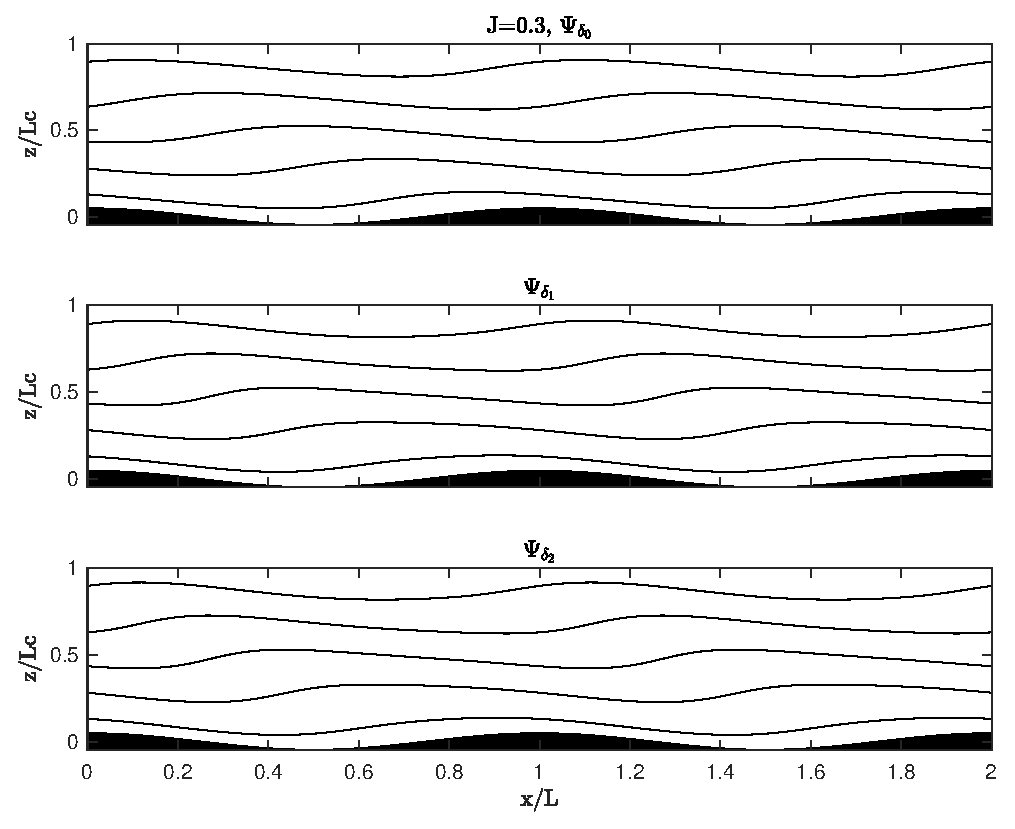
\includegraphics[width=1\textwidth]{delta_solutions.eps}
	\caption{0th, 1st, and 2nd order solutions for $\delta(x,z)$ with $J=0.3$.}
\end{figure}

\begin{figure}
	\centering
	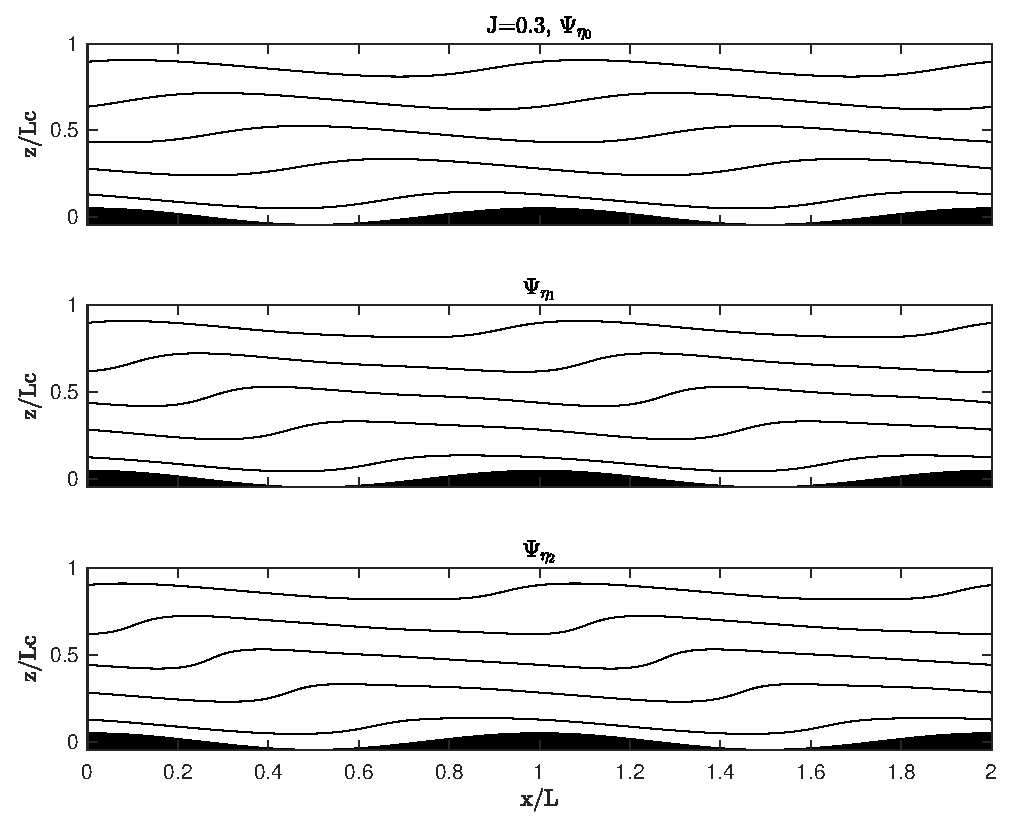
\includegraphics[width=1\textwidth]{eta_solutions.eps}
	\caption{0th, 1st, and 2nd order solutions for $\eta(x,z_0)$ with $J=0.3$.}
\end{figure}

\begin{figure}
	\centering
	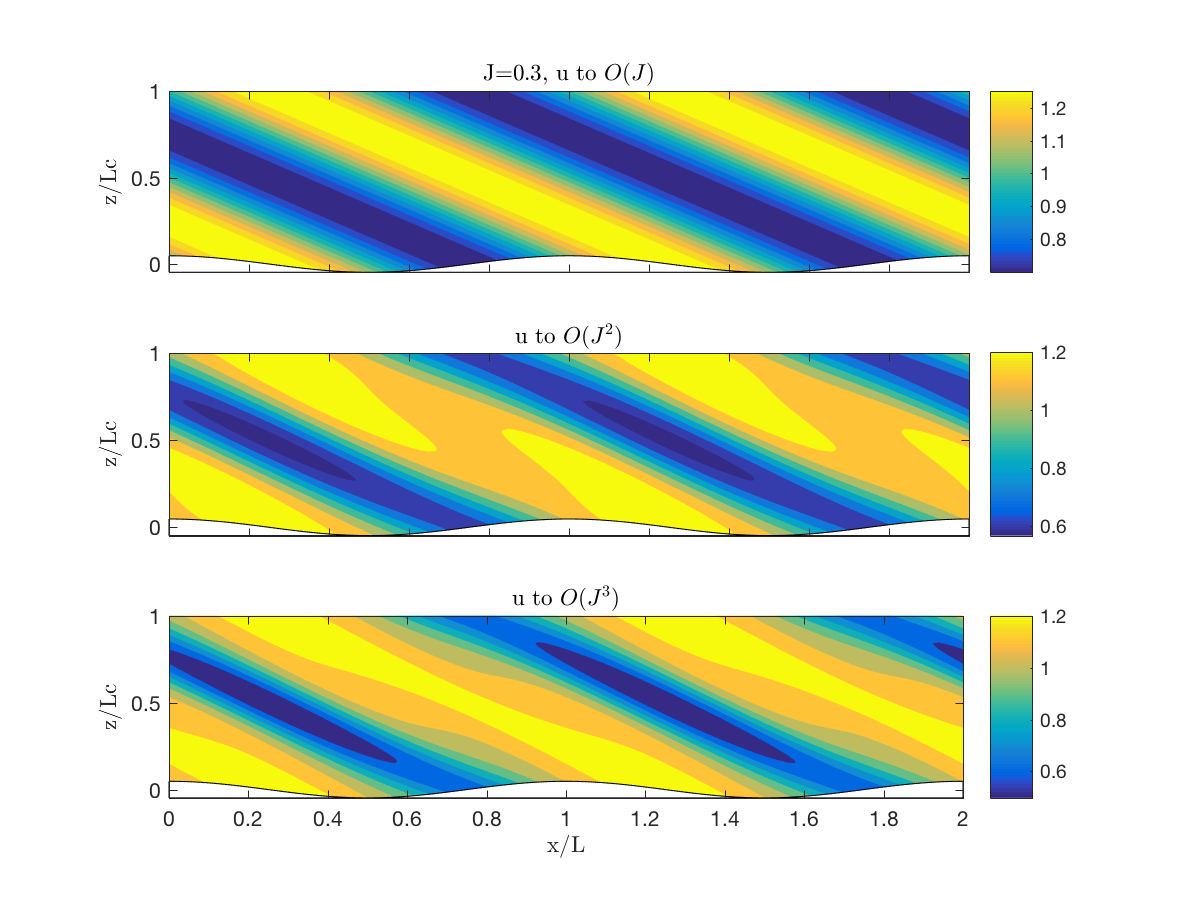
\includegraphics[width=1\textwidth]{u_solutions.eps}
	\caption{0th, 1st, and 2nd order solutions for $u(x,z_0)$ with $J=0.3$.}
\end{figure}

\begin{figure}
	\centering
	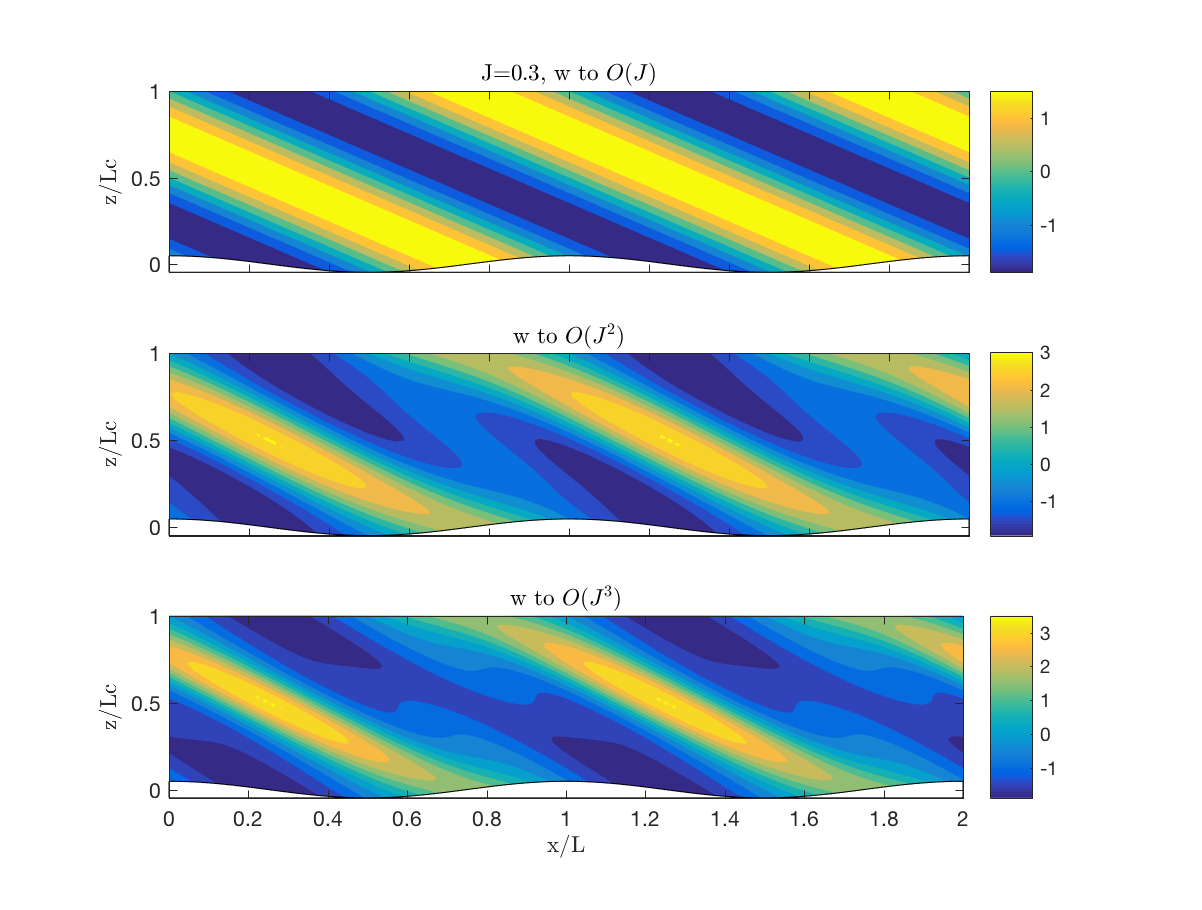
\includegraphics[width=1\textwidth]{w_solutions.eps}
	\caption{0th, 1st, and 2nd order solutions for $w(x,z_0)$ with $J=0.3$.}
\end{figure}

\begin{figure}
	\centering
	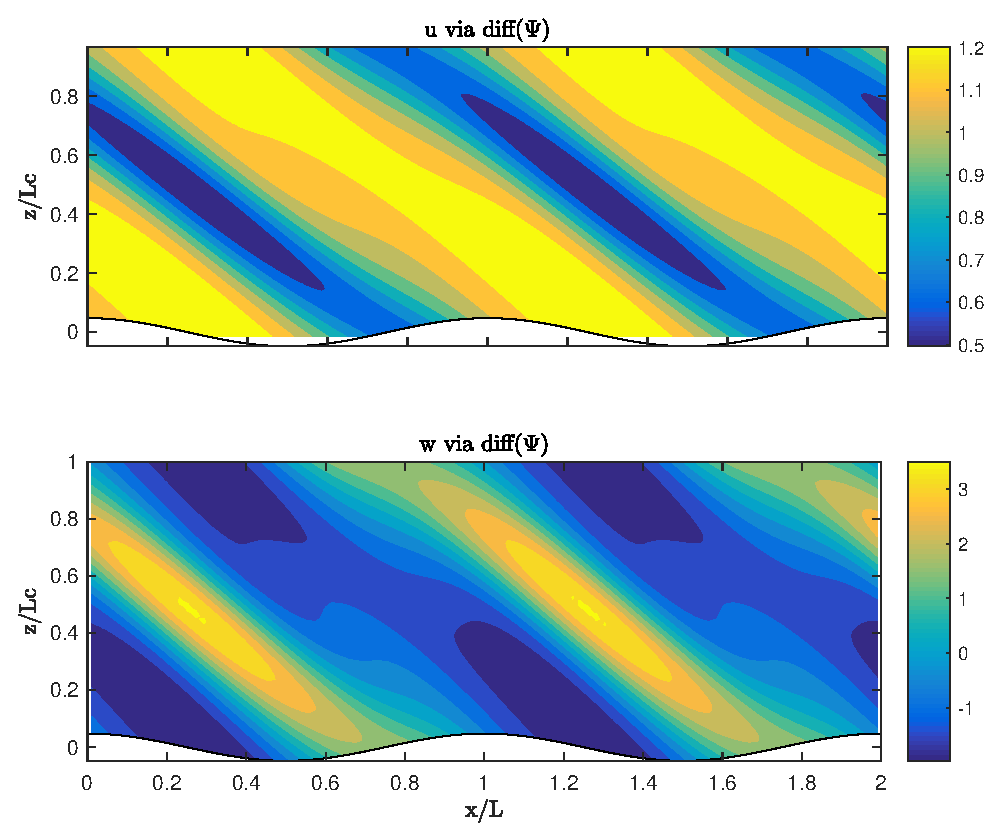
\includegraphics[width=1\textwidth]{vel_via_diff.eps}
	\caption{2nd order solutions for velocity calculated by numerical differentiation of $\eta_2$.}
\end{figure}

\subsection{Instability}

These if taken to large enough order, these perturbation expansions are asymptotically exact so long as $J<1$. However, before $J$ gets to unity, these solutions suggest that two forms of instability will arise, invalidating the underlying hypothesis of Long's model. 

Firstly, as $J$ increases, the streamlines steepen, and at some value of $J<1$, become locally vertical. Vertical streamlines imply wave breaking (Long 1953, Miles 1969) which results in heavy water pooling in valleys and reduced wave amplitude (Kimura and Manins 1980). The condition of vertical streamlines can be expressed mathematically as $\partial_z \delta = 1$. 

Below, I include a plot of the maximum value of $\partial_z \delta$ as a function of J for each order solution. As Smith reported in 1977, the 1st order accurate solution for $\delta$ predicts that wave breaking will commence at $J=0.75$. With our next order solution, this threshold drops to $J=0.65$. Of course, neither solutions are suitable for analysis of such nonlinear flow; in order to limit the error in a $J=0.65$ solution to less than $5\%$, we would need a 6th order accurate expansion ($0.65^7 = 0.049$). 

A second measure of instability derives from consideration of turbulent energetics, and is quantified by the  a condition on $Ri = N^2/(\partial_z u)^2$, where $Ri$ is the Richardson number and is a ratio of the  contributions of buoyancy flux and shear production  to the turbulent kinetic energy equation. If $Ri>1/4$, buoyancy will not allow the energy cascade to perpetuate, and the flow stabilizes. However, if $Ri<1/4$, vertical shear wins and the flow collapses into turbulence (Miles 1961, Baines 1995). 

Note that from our scaling above, we have $u_0 = JU$, $\partial_z = N/U$, and together $(\partial_z u)^2 \propto N^2J^2$ and $Ri \propto J^{-2}$. Thus we expect the flow to go unstable at least by $J=2$. To get at this more quantitatively, however, consider the vertical gradient of our perturbation solutions for $u$, plotted as a function of J below. I find (numerically), that in the $O(J^6)$ solution (recall, it is a square of the gradient of $u$, which we have solved to $O(J^2)$), Ri falls below 1/4 for $J>0.69$. Furthermore, because of the higher order of this solution, the error in this estimate is much more acceptable than for the vertical streamlines ($0.69^7=0.0745$).


\begin{figure}
	\centering
	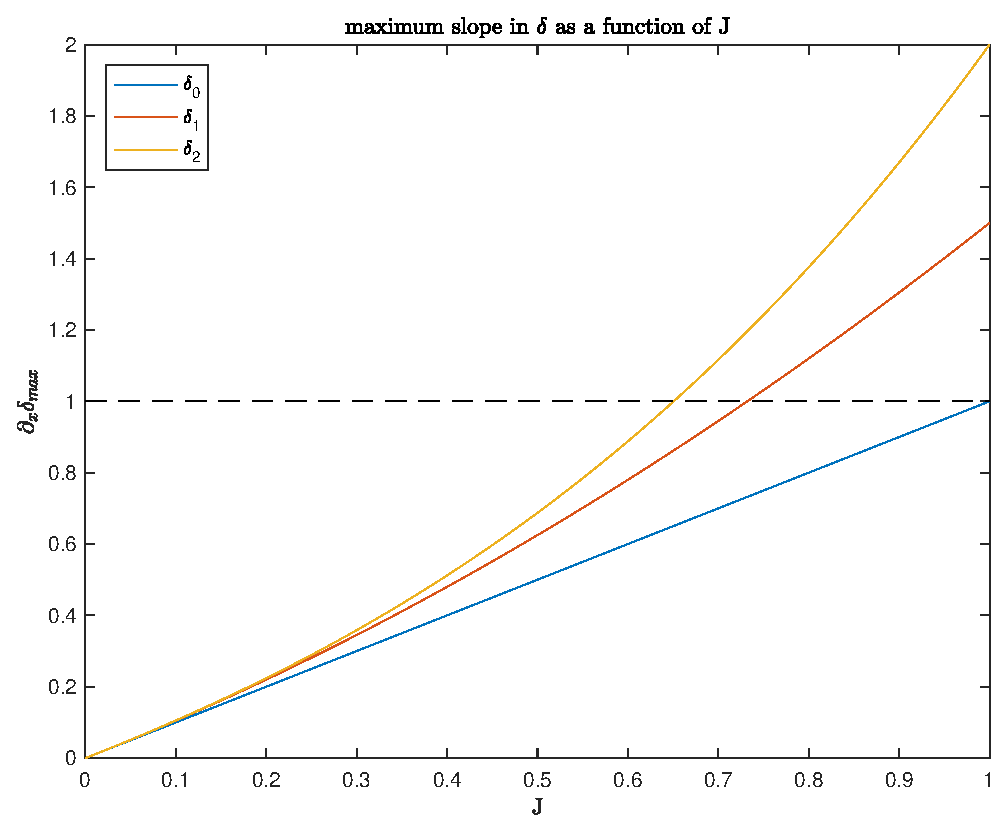
\includegraphics[width=1\textwidth]{max_slopes.eps}
	\caption{Maximum slope in $\delta$ as a function of J.}
\end{figure}

\begin{figure}
	\centering
	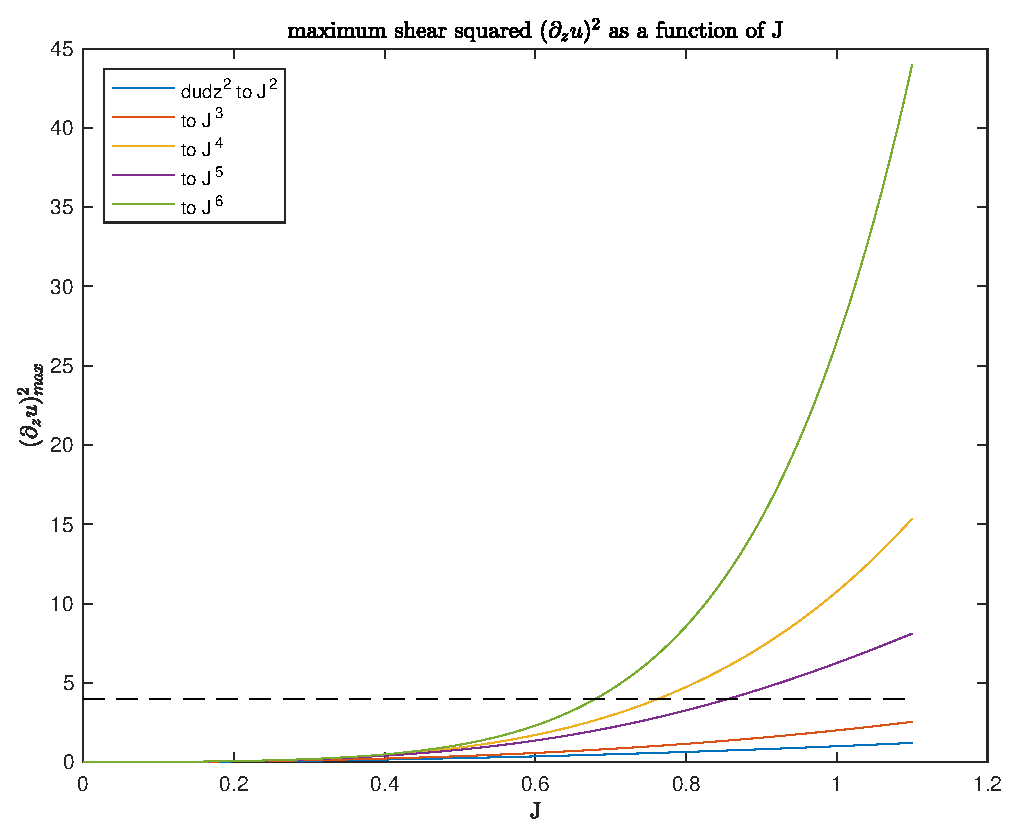
\includegraphics[width=1\textwidth]{max_shearsq.eps}
	\caption{Maximum slope in $(\partial_z u)^2$ as a function of J.}
\end{figure}

\subsection{Momentum and Energy fluxes}
The generation of a lee wave represents a transfer of momentum and energy from the mean flow into the perturbation flow. This transfer initiates at the bottom boundary, where it is felt as a form drag. The fluxes then radiate upwards with the wave, to infinity as far as this problem is concerned. 

The horizontal force of the topography on the mean flow from the pressure gradient at the surface is 
\[
F_D =  \int \D{P}{x} h(x) dx = -\int P(x) \D{h}{x} dx.
\]
Using the work energy theorem, the energy expended in flowing over the topography is then
\[
E_D = -\int u(x)P(x) \D{h}{x} dx.
\]
Away from the hill, the wave momentum flux is
\[
F_w(x,z_0) = -\rho u(z,x_0)w(x,z_0),
\]
and the wave energy flux is
\[
E_w(x,z_0) = P(x,z_0)w(x,z_0).
\]
For our inviscid and irrotational problem, there is no energy lost or converted to inertial oscillations while fluxing through the domain, and $E_D = E_w$.

To evaluate these fluxes, it will be helpful to have a clear relation between the pressure field and $\eta(x,z_0)$.

\subsection{Fourier synthesis}


\begin{figure}
	\centering
	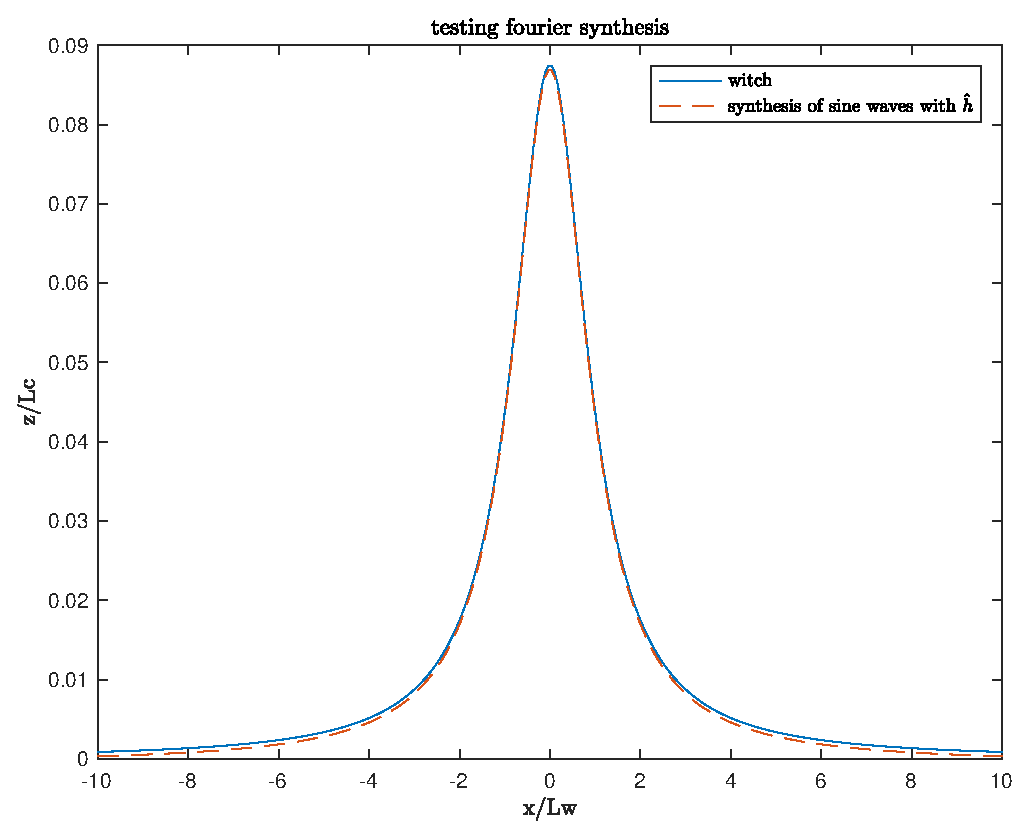
\includegraphics[width=1\textwidth]{witch_bathymetry.eps}
	\caption{Recreating the Witch of Agnesi using Fourier synthesis.}
\end{figure}

\begin{figure}
	\centering
	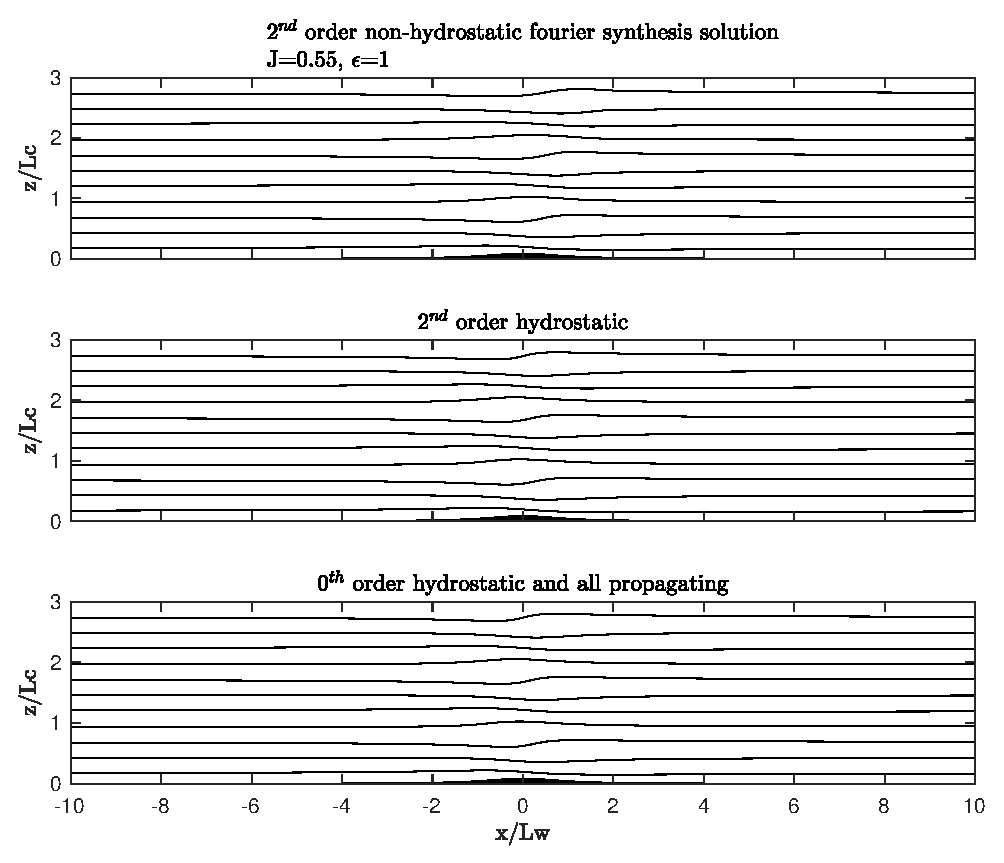
\includegraphics[width=1\textwidth]{witch_eta.eps}
	\caption{Streamlines above a Witch of Agnesi found via Fourier synthesis.}
\end{figure}

\end{document}




w = cos(x)exp(-m z)
wx = -sin(x)exp(-m z)
ux = -wz = m cos(x) exp(-m z)
u = m sin(x) exp(-m z)

rhox = w = cos(x)exp(-m z)
rho = sin(x)exp(-m z)

e2 wx = -pz - rho
pz = -e2 wx - rho = e2 sin(x) exp(-m z) - sin(x) exp(-m z) = m^2 sin(x) exp(-m z)
p = (-1/m) m^2 sin(x) exp(-m z) = -m sin(x) exp(-m z)



